% \documentclass[12pt, twoside]{article}
\usepackage[letterpaper, margin=1in, headsep=0.2in]{geometry}
\setlength{\headheight}{0.6in}
%\usepackage[english]{babel}
\usepackage[utf8]{inputenc}
\usepackage{microtype}
\usepackage{amsmath}
\usepackage{amssymb}
%\usepackage{amsfonts}
\usepackage[nomessages]{fp} %\FPeval{\var-name}{2*sin(pi/6)}
\usepackage{siunitx} %units in math. eg 20\milli\meter
\usepackage{yhmath} % for arcs, overparenth command
\usepackage{tikz} %graphics
\usetikzlibrary{quotes, angles, arrows, arrows.meta}
\usepackage{graphicx} %consider setting \graphicspath{{images/}}
\usepackage{parskip} %no paragraph indent
\usepackage{enumitem}
\usepackage{multicol}
\usepackage{venndiagram}

\usepackage{fancyhdr}
\pagestyle{fancy}
\fancyhf{}
\renewcommand{\headrulewidth}{0pt} % disable the underline of the header
\raggedbottom
\hfuzz=2mm %suppresses overfull box warnings

\usepackage{hyperref}

\fancyhead[LE]{\thepage}
\fancyhead[RO]{\thepage \\ Name: \hspace{4cm} \,\\}
\fancyhead[LO]{BECA / Dr. Huson / Geometry\\*  Unit 2: Angles\\* 6 October 2022}

\begin{document}

\subsubsection*{2.7 Test: Extension topics}
\emph{Diagrams are not necessarily drawn to scale unless otherwise stated.}
\begin{enumerate}

\item The protractor shown below is marked with degree measures on the inside and radian measures on the outside. Make a 1 radian angle by drawing a ray from the center $V$ through the protractor semicircle. \par \medskip
  \begin{center}
  \begin{tikzpicture}
    \draw[thick] (-3,0)--(0,0)--(3,0);
    \draw (4,0) arc (0:180:4);
    \fill (0,0) circle [radius=0.05]node[below]{$V$};
    \foreach \x in {0,15,30,...,180}
      \node at (\x:3.4){\x};
    \foreach \x in {0,15,30,...,180}
      \draw (\x:3.7)--(\x:4);
    \foreach \x in {0,5,...,180}
      \draw (\x:3.9)--(\x:4);
    \foreach \x in {0,0.1,...,3.1}
      \draw (57.3*\x:4)--(57.3*\x:4.3);
    \foreach \x in {0.2,0.4,0.6,0.8,1.0,1.2,1.4,1.6,1.8,2.0,2.2,2.4,2.6,2.8,3.0}
      \node at (57.3*\x:4.7){\x};
    \draw (-4.3,0)node[left]{$\pi$}--(-4,0);
    \draw[->,thick] (4,0)--(0:6);
    \end{tikzpicture}
  \end{center}

\item Use the protractor above to convert radians and degrees. (nearest whole degree, nearest hundredth radian).\vspace{.25cm}
  \begin{multicols}{2}
    \begin{enumerate}
      \item $80^\circ = $ \vspace{0.7cm}
      \item $28^\circ = $ \vspace{0.7cm}
      \item $\displaystyle 1.0 \text{ radian} =$ \vspace{0.7cm}
      \item $\displaystyle 2.7 \text{ radian} =$
    \end{enumerate}
  \end{multicols} \vspace{1cm}

\newpage
\item In the diagram below $\angle BOC = 7x-50$ and $\angle DOE = 4x-3$. Find m$\angle AOB$. \vspace{0.25cm}
\begin{flushright}
\begin{tikzpicture}[scale=1.3, rotate=-20]
  \draw[<->, thick] (-40:3)--(0,0)--(140:3);
  \draw[<->, thick] (-3,0)--(3,0);
  \draw[->, thick] (0,0)--(0,3);
  \draw (0,0)++(0.3,0)--++(0,0.3)--+(-0.3,0);
  \draw[fill] (140:2) circle [radius=0.05] node[below left]{$B$};
  \draw[fill] (-2,0) circle [radius=0.05] node[below]{$A$}; 
  \draw[fill] (0,0) circle [radius=0.05] node[below left]{$O$};
  \draw[fill] (0,2) circle [radius=0.05] node[left]{$C$};
  \draw[fill] (2,0) circle [radius=0.05] node[below]{$D$};
  \draw[fill] (-40:2) circle [radius=0.05] node[left]{$E$};
\end{tikzpicture}
\end{flushright}

\item In the diagram below $\angle AOB = x-7$ and $\displaystyle \angle COD = \frac{3}{4}(x+57)$. Find $\angle BOC$ \vspace{0.25cm}
\begin{flushright}
\begin{tikzpicture}[scale=1, rotate=0]
\draw[->, thick] (0,0)--(155:5);
\draw[<->, thick] (-5,0)--(5,0);
\draw[->, thick] (0,0)--(0,4);
\draw (0,0)++(0.3,0)--++(0,0.3)--+(-0.3,0);
\draw[fill] (155:3) circle [radius=0.05] node[below left]{$B$};
\draw[fill] (-4,0) circle [radius=0.05] node[below]{$A$}; 
\draw[fill] (0,0) circle [radius=0.05] node[below]{$O$};
\draw[fill] (0,3) circle [radius=0.05] node[left]{$C$};
\draw[fill] (4,0) circle [radius=0.05] node[below]{$D$};
\end{tikzpicture}
\end{flushright}

\newpage
\item In the line segment $\overline{ABC}$, $\overline{AB}$ is twice as long as $\overline{BC}$. $AB=12x-6$ and $AC=15x+9$. Find $BC$.
\vspace{5cm}

\end{enumerate}
\end{document}